% Shared preamble for the English summaries in this repository.
\documentclass[11pt,a4paper]{article}
\usepackage[margin=2.2cm]{geometry}
\usepackage[T1]{fontenc}
\usepackage[utf8]{inputenc}
\usepackage{lmodern}
\usepackage{amsmath,amssymb}
\usepackage{graphicx}
\usepackage{booktabs}
\usepackage{enumitem}
\usepackage[hidelinks]{hyperref}
\setlist{itemsep=2pt,topsep=4pt}
\setlength{\parindent}{0pt}
\setlength{\parskip}{5pt}
\graphicspath{{figures/}}
\newcommand{\summaryheader}[3]{%
  \begin{center}
    {\Large\bfseries #2}\\[3pt]
    {\large #1}\\[3pt]
    {\small Arshia Goshtasbi \textbullet{} MSc Electrical Engineering (Control), Iran University of Science and Technology \textbullet{} #3}
  \end{center}
  \vspace{2pt}\hrule\vspace{8pt}\par}

\begin{document}
\summaryheader{Machine Learning, Homework 6}{Neural Networks: Back-propagation by Hand and MLPs in PyTorch}{Spring 1404 (2025)}

\textbf{Notebook} (\texttt{mlp\_mnist\_cifar10.ipynb}; the outputs are from my original run on Colab).
\begin{itemize}
  \item \emph{MNIST.} I built the data pipeline (tensor conversion, normalisation, data loaders) and an MLP $784\to128\to10$ with ReLU (101{,}770 parameters). I trained it with Adam for 5 epochs; the training loss fell from $0.38$ to $0.10$ and the test accuracy is $96.6\%$.
  \item \emph{CIFAR-10.} I trained a single linear layer $3072\to10$ (a softmax perceptron, 30{,}730 parameters) with SGD for 10 epochs. It reaches $37.6\%$ test accuracy, which shows the limit of a linear model on natural images (Figure~\ref{fig:cifar}).
\end{itemize}

\begin{figure}[h]\centering
  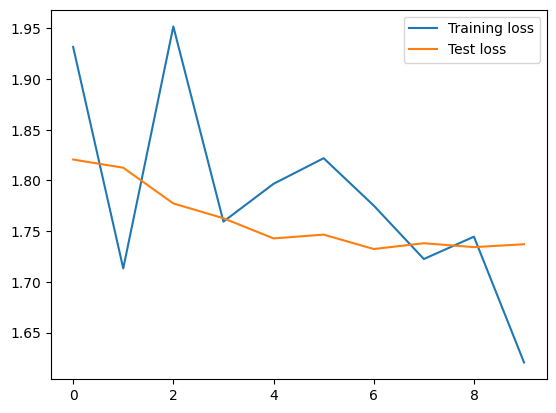
\includegraphics[width=.45\linewidth]{mlp_mnist_cifar10_cell41_1.png}\hfill
  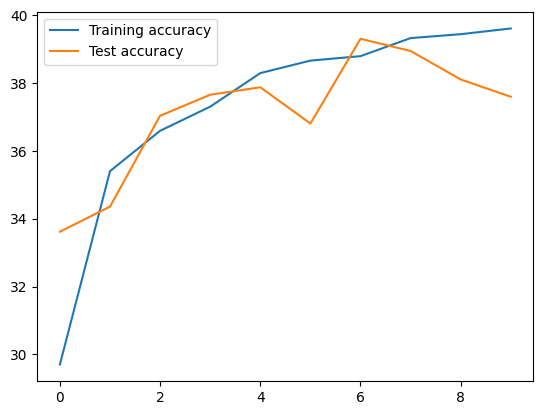
\includegraphics[width=.45\linewidth]{mlp_mnist_cifar10_cell44_1.png}
  \caption{CIFAR-10 linear classifier: loss (left) and accuracy in \% (right) per epoch.}\label{fig:cifar}
\end{figure}

\textbf{Written part.}
\begin{description}
  \item[Moving a point between K-means clusters.] I showed that removing $\tilde x$ from cluster $i$ changes its cost to $J_i^+=J_i^--\frac{N_i^-}{N_i^--1}\|\tilde x-\mu_i^-\|^2$, and that adding it to cluster $j$ gives $J_j^+=J_j^-+\frac{N_j^-}{N_j^-+1}\|\tilde x-\mu_j^-\|^2$. This is the test for whether a move lowers the total cost.
  \item[Computational graph.] For $z=wx+b$, $y=\sigma(z)$, $\mathcal L=\tfrac12(y-t)^2$ and $\mathcal L_{\mathrm{reg}}=\mathcal L+\tfrac\lambda2\|w\|^2$, I drew the graph and back-propagated: $\bar y=y-t$, $\bar z=\bar y\,\sigma(z)(1-\sigma(z))$, $\bar w=\bar z\,x+\lambda w$, $\bar b=\bar z$. I then ran one gradient step by hand with $w=0.5$, $b=0.1$, $x=1$, $t=0.8$, $\lambda=0.01$ and $\eta=0.1$.
  \item[Initialisation.] Equal weights never break symmetry, so all hidden units stay the same. Large weights saturate sigmoid/tanh units (vanishing gradients) or make gradients explode in deep networks. Weights that are too small make the signal fade.
  \item[Twin network.] I derived the partial derivatives of the cross-entropy cost for a weight-sharing (Siamese) network, and the update rule with $L_2$ regularisation.
\end{description}
\end{document}
